%Cap4a 31
\begin{frame}{Heurísticas admisibles}
E.g., para el puzle-8: \newline
\textcolor{pink}{$h_1(n) = $}  número de fichas que están en la posición incorrecta.\newline
\textcolor{pink}{$h_2(n) = $}  distancia Manhattan total.\newline
(i.e., número de cuadrados desde la posición deseada de cada ficha)
    \begin{figure}[h]
        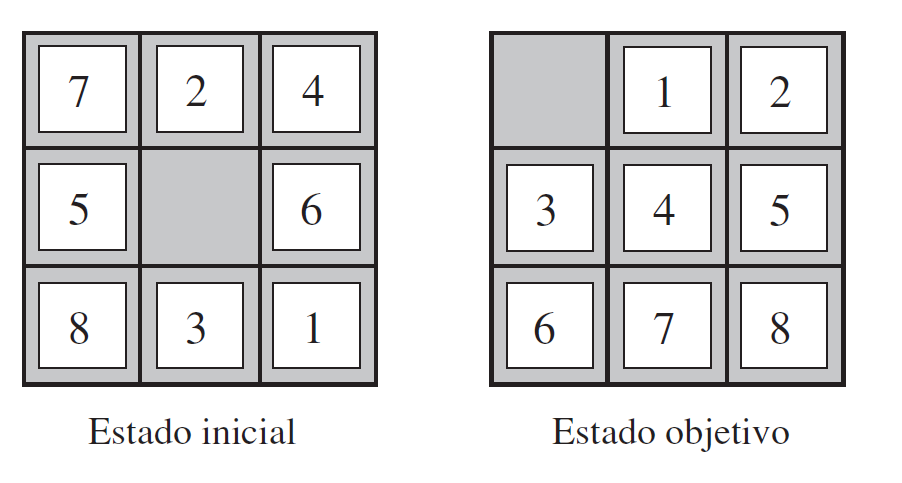
\includegraphics[scale = 0.2]{4a_puzle8.png}
    \end{figure}
\textcolor{pink}{$h_1(n) = ??$}\newline
\textcolor{pink}{$h_2(n) = ??$}
\end{frame}
